\chapter{Tipps für \LaTeX}\label{latex}

Hier finden Sie gesammelte Hinweise, die sich speziell auf das \LaTeX-Template und dessen Verwendung beziehen. Der Aufbau des Templates wird dargelegt und wichtige Befehle werden anhand von Beispielen erklärt.

\section{Struktur des Templates}

\begin{description}
    \item[mi-document/]{Dieses Verzeichnis enthält die Style- und Class-Files, die das eigentliche Template darstellen. In diesen werden Pakete importiert, Formatierungen definiert und zusätzliche Funktionen bereitgestellt. Manche Entwicklungsumgebungen für \LaTeX, wie TeXmaker und TeXstudio, finden diese Dateien leider nur, wenn sie sich im gleichen Verzeichnis befinden wie \verb|document.tex|. In diesem Fall müssen alle \verb|.sty|- und \verb|.cls|-Dateien in dessen Verzeichnis verschoben werden.}
    \item[document.tex]{Diese Datei enthält den Quellcode für dieses Dokument. Es wird empfohlen, Arbeiten auf diese Datei aufzubauen. In den ersten Zeilen werden Variablen definiert (z.B. Autor, Titel der Arbeit, etc.), welche vom Template beispielsweise für das Deckblatt und Metadaten verwendet werden. Danach werden Inhalts-, Abbildungs-, Tabellen- und Codeverzeichnis angezeigt. Der tatsächliche Inhalt der Arbeit kann direkt in diese Datei geschrieben werden, es wird jedoch empfohlen, Kapitel auf verschiedene Dateien aufzuteilen und über den \verb|\input|-Befehl einzubinden.}
    \item[lizenzierung.tex]{Hier werden Lizenzen für die schriftliche Ausarbeitung und den Code der Arbeit sowie ein eventueller Sperrvermerk (nur nach Absprache!) angegeben. Passen Sie diese Datei so an, dass sie auf Ihre Arbeit zutrifft. Mit den Befehlen \verb|\checkboxEmpty| und \verb|\checkboxChecked| können leere und angekreuzte Kästchen erstellt werden.}
    \item[hinweise.tex]{Diese Datei enthält die Präambel dieser Formatvorlage und sollte \textbf{nicht} in Ihrer fertigen Arbeit enthalten sein. Entfernen Sie dazu den Import dieser Datei aus \verb|document.tex|.}
    \item[*.tex]{Die anderen \verb|.tex|-Dateien enthalten den Inhalt dieses Dokuments (eine Datei pro Kapitel). Sie werden von \verb|document.tex| importiert.}
    \item[images/]{Bilddateien in diesem Verzeichnis können als Abbildungen in ein \LaTeX-Dokument eingebunden werden.}
\end{description}

\section{Wichtige Befehle}

\subsection{Sections, Subsections, etc.}

Die Abschnitte eines \LaTeX-Dokuments werden in \emph{chapters}, \emph{sections} und \emph{subsections} aufgeteilt.
Diese Abschnitte werden automatisch mit einer fortlaufenden Nummerierung versehen und im Inhaltsverzeichnis aufgeführt.
Die Syntax der Befehle lautet wie folgt:

\begin{lstlisting}[language=TeX]
\chapter{Kapitelname}              % z.B. 4 Gestaltungsrichtlinien
\section{Unterkapitelname}         % z.B. 4.3 Formatierung
\subsection{Unterunterkapitelname} % z.B. 4.3.3 Abbildungen
\end{lstlisting}

Es wir empfohlen, Abschnitte außerdem mit Labels zu versehen, damit sie im späteren Verlauf der Arbeit einfacher referenziert werden können:

\begin{lstlisting}[language=TeX]
\chapter{Kapitelname}\label{sec:Kapitelname} % Label wird gesetzt
\ref{sec:Kapitelname}                        % Referenz auf das Label
\end{lstlisting}

Das die Referenz wird im Fließtext durch die \textbf{Kapitelnummer} ersetzt, sodass eine Syntax wie \verb|(siehe Kapitel \ref{Kapitelname})| empfohlen wird.

Ist ein Abschnitt \textbf{ohne} Nummerierung gewünscht, so können die Befehle \verb|\addchap| und \verb|\addsec| genutzt werden. Diese erzeugen nicht-nummerierte Überschriften inklusive Eintrag ins Inhaltsverzeichnis.

Darüber hinaus existieren noch kleinere Zwischen-Überschriften, die nicht in das Inhaltsverzeichnis eingetragen werden.

\begin{lstlisting}[language=TeX]
\minisec{Überschrift}
\end{lstlisting}



\subsection{Listen}

\LaTeX{} stellt drei verschiedene Arten von Listen bereit: Aufzählungen \emph{(itemize)}, nummerierte Aufzählungen \emph{enumerate} und Beschreibungen \emph{description}.
Beispielhaft werden hier Quellcode und Resultat dargestellt:

\minisec{Aufzählung}

\begin{lstlisting}[language=TeX]
\begin{itemize}
    \item{Das ist der erste Punkt.}
    \item{Das ist der zweite Punkt.}
    \item{Das ist der dritte Punkt.}
\end{itemize}
\end{lstlisting}

\begin{itemize}
    \item{Das ist der erste Punkt.}
    \item{Das ist der zweite Punkt.}
    \item{Das ist der dritte Punkt.}
\end{itemize}

\minisec{Nummerierte Aufzählung}

\begin{lstlisting}[language=TeX]
\begin{enumerate}
    \item{Das ist der erste Punkt.}
    \item{Das ist der zweite Punkt.}
    \item{Das ist der dritte Punkt.}
\end{enumerate}
\end{lstlisting}

\begin{enumerate}
    \item{Das ist der erste Punkt.}
    \item{Das ist der zweite Punkt.}
    \item{Das ist der dritte Punkt.}
\end{enumerate}

\minisec{Beschreibung}

\begin{lstlisting}[language=TeX]
\begin{description}
    \item[Erstens]{Das ist der erste Punkt.}
    \item[Zweitens]{Das ist der zweite Punkt.}
    \item[Drittens]{Das ist der dritte Punkt.}
\end{description}
\end{lstlisting}

\begin{description}
    \item[Erstens]{Das ist der erste Punkt.}
    \item[Zweitens]{Das ist der zweite Punkt.}
    \item[Drittens]{Das ist der dritte Punkt.}
\end{description}

\noindent Unterpunkte können erstellt werden, indem innerhalb einer Liste eine neue Liste erstellt wird:

\begin{lstlisting}[language=TeX]
\begin{itemize}
    \item{Das ist der erste Punkt.}
    \item{Das ist der zweite Punkt.}
    \begin{itemize}
        \item{Das ist ein Unterpunkt.}
        \item{Das ist noch ein Unterpunkt.}
    \end{itemize}
\end{itemize}
\end{lstlisting}

\begin{itemize}
    \item{Das ist der erste Punkt.}
    \item{Das ist der zweite Punkt.}
    \begin{itemize}
        \item{Das ist ein Unterpunkt.}
        \item{Das ist noch ein Unterpunkt.}
    \end{itemize}
\end{itemize}

\subsection{Abbildungen, Tabellen und Code}

Größere Objekte, wie Tabellen oder Bilder, sollten in der Regel nicht an einer festen Position platziert werden.
Der Seitenumbruch kann sonst nicht optimal platziert werden und bei der Platzierung mitten auf der Seite, wird der Lesefluss unterbrochen.
\LaTeX{} liefert hier dem Autor die Möglichkeit sogenannte \emph{Gleitobjekte} mithilfe einer \emph{Gleitumgebung} zu definieren.

Dies führt dazu, dass Objekte möglichst sinnvoll platziert werden, jedoch nicht direkt an der Stelle, an der sie definiert wurden, vgl. Abbildung \ref{fig:beispiel}.
Die nicht-exakte Positionierung des Objektes ist dabei kein Nachteil, da ohnehin jede Abbildung über eine entsprechende Beschriftung und Nummer verfügen muss.
Dadurch ist die Zuordnung mithilfe von Querverweisen möglich.

Die Gleitumgebung heißt für Abbildungen \emph{figure} und für Tabellen \emph{table}. Die folgenden Mechanismen sind dabei analog benutzbar, es ändert sich lediglich der Bezeichner an der Beschriftung.

\begin{lstlisting}[language=TeX]
\begin{figure}
<hier wird das eigentliche Bild eingefügt, siehe Folgeabschnitt>
\caption{Bildbeschreibung}
\label{fig:label}
\end{figure}
\end{lstlisting}


Der Querverweis auf die Abbildung ist dann folgendermaßen möglich:
\begin{lstlisting}[language=TeX]
siehe Abbildung \ref{fig:beispiel}
\end{lstlisting}
es erzeugt die Ausgabe: „siehe Abbildung \ref{fig:beispiel}“

Alle Gleitumgebungen verfügt zusätzlich über ein Optionales Argument, dass zur Beeinflussung der Platzierung benutzt werden kann:
\begin{lstlisting}[language=TeX]
\begin{figure}[Platzierung „tbp“, falls nicht angegeben]
\end{lstlisting}

Dieses Argument kann eine Prioritätenliste aus t „top“, b „bottom“, h „here“ oder p „page“ (extra
Seite) gesetzt werden. Der erste Wert der Liste hat die höchste Priorität und wird wenn möglich verwirklicht.
Voreingestellt ist tbp. Dies ist dadurch begründet, dass h eine Positionierung mitten auf der Seite
bedeutet. Die daraus resultierende Spaltung des Satzspiegels ist typografisch fragwürdig und wird daher nicht empfohlen.


\minisec{Abbildungen}

Um eine Abbildung einzufügen kann obiges Beispiel entsprechend erweitert werden:

\begin{lstlisting}[language=TeX]
\begin{figure}
	\centering
	\includegraphics[width=0.5\textwidth]{images/dateiname}
	\caption{Bildbeschreibung}
	\label{fig:label}
\end{figure}
\end{lstlisting}

\begin{figure}
	\centering
	\includegraphics[width=0.5\textwidth]{images/blume}
	\caption{Bildbeschreibung des Beispielbildes}
	\label{fig:beispiel}
\end{figure}

Meist sind ausführliche Bildbeschreibungen empfehlenswert, damit eine Abbildung für sich selbst stehen kann.
In diesem Fall kann durch einen optionalen Parameter \verb|\caption[Kurzbeschreibung]{Langbeschreibung}| eine Kurzform angegeben werden, welche dann im Abbildungsverzeichnis erscheint.

\begin{wrapfigure}{R}{0.3\textwidth}
	\centering
	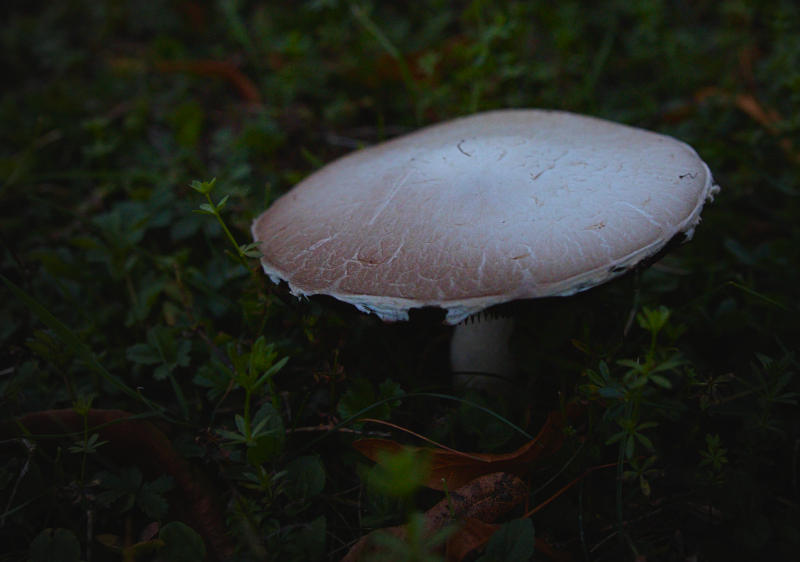
\includegraphics[width=0.25\textwidth]{images/schwammerl}
	\caption{Bild mit Textumfluss.}
	\label{fig:beispiel_umfluss}
\end{wrapfigure}

Bei sehr hohen und schmalen Bildern kann es nützlich sein, Textumfluss zu verwenden.
Dies kann in \LaTeX mit der \verb|wrapfigure|-Umgebung umgesetzt werden:

\begin{lstlisting}[language=TeX]
\begin{wrapfigure}{R}{0.3\textwidth}
	\centering
	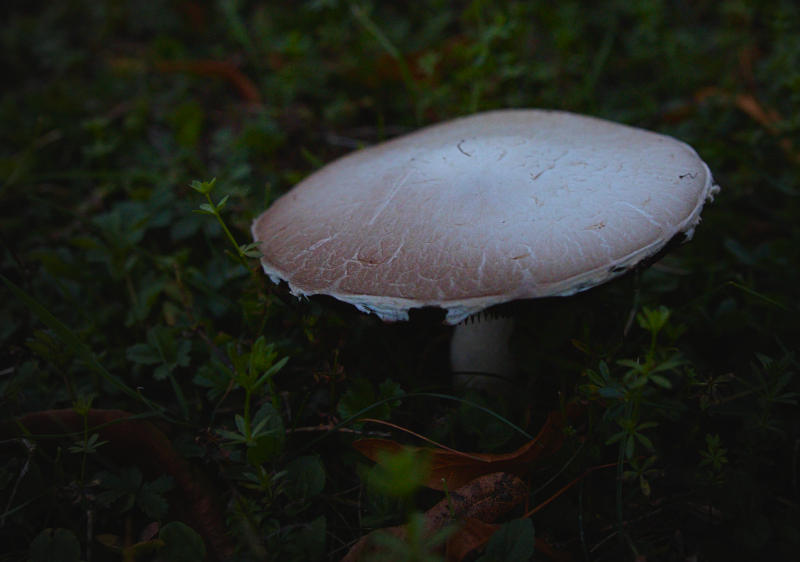
\includegraphics[width=0.25\textwidth]{images/schwammerl}
	\caption{Bild mit Textumfluss.}
	\label{fig:beispiel_umfluss}
\end{wrapfigure}
\end{lstlisting}



Falls Ihre Arbeit viele Abbildungen des gleichen Formates enthält, können Sie sich folgendermaßen ein Makro als Abkürzung definieren:

\begin{lstlisting}[language=TeX]
\newcommand*{\image}[2]{
	\begin{figure}
	\centering
	\includegraphics[width=0.5\textwidth]{images/#1}
	\caption{#2}
	\label{fig:#1}
	\end{figure}
}
\end{lstlisting}
Diese Definition steht in der Datei \emph{config.tex} und kann dort auch angepasst werden.

Damit erhalten Sie die Möglichkeit statt der obigen Umgebung einfach
\begin{verbatim}
\image{dateiname}{Bildbeschreibung}
\end{verbatim}
zu benutzen. Das Label erhält in diesem Fall den Namen „fig:<Dateiname>” für das Beispielbild.

\image{blume}{zweite Verwendung des Beispielbildes mit dem image-Makro. Die Datei heißt blume.jpg.}

Die Referenz \ref{fig:blume} wird dann mit \verb+\ref{fig:blume}+ erzeugt.

\minisec{Tabellen}

Tabellen in \LaTeX{} zu erstellen mag anfangs etwas umständlich erscheinen, sie bieten jedoch sehr viel gestalterische Möglichkeiten. Hier werden lediglich die einfachsten Grundlagen gezeigt.

Für die Platzierung kann, wie zu Beginn dieses Abschnittes Beschrieben die \emph{table}-Umgebung benutzt werden.

Innerhalb dieser befindet sich mit dem \emph{tabular}-Environment die eigentliche Tabelle.
Dessen Parameter bestimmen die Anzahl der Spalten, sowie die Ausrichtung der Inhalte dieser.
Über \verb|\hline| können horizontale Linien eingebaut werden.
Die Inhalte werden Zeilenweise (getrennt durch \verb|\\|) hinzugefügt und diese Zeilen werden durch das \verb|&|-Symbol in Spalten unterteilt.

Die Anpassung des Makros \verb+\arraystretch+ erhöht den Zeilenabstand. Für elegantere Lösungen betreffend Tabellen sei auf Ergänzungspakete wie tabularx \citep{latex:tabularx} oder booktabs \citep{latex:booktabs} verwiesen.

\begin{lstlisting}[language=TeX]
\begin{table}
\renewcommand{\arraystretch}{1.5}
\centering
\begin{tabular}{l|l}
\hline
\bfseries Erste Spalte& \bfseries Zweite Spalte \\
\hline
Erste Zeile & lorem \\
Zweite Zeile & ipsum \\
Dritte Zeile & dolor \\
\hline
\end{tabular}
\caption{Tabellenbeschreibung}
\label{table:label_der_tabelle}
\end{table}
\end{lstlisting}

\begin{table}
	\renewcommand{\arraystretch}{1.5}
	\centering
	\begin{tabular}{l|l}
		\hline
		\bfseries Erste Spalte& \bfseries Zweite Spalte \\
		\hline
		Erste Zeile & lorem \\
		Zweite Zeile & ipsum \\
		Dritte Zeile & dolor \\
		\hline
	\end{tabular}
	\caption{Tabellenbeschreibung}
	\label{table:label_der_tabelle}
\end{table}

\minisec{Code}

Um Code einzubinden, wird das \verb|lstlisting|-Environment verwendet.
Über Parameter können Metadaten wie die Programmiersparche (wichtig für korrektes Syntax-Highlighting), die Beschreibung und das Label festgelegt werden.

\begin{verbatim}
\begin{lstlisting}[language=C++,
                   caption={Beschreibung des Codebeispiels},
                   captionpos=b,
                   label=code:code_label]
#include <stdio.h>

int main()
{
    printf("Hallo Welt!\n");
}
\end{lstlisting}
\end{verbatim}

\begin{lstlisting}[language=C++,
                   caption={Beschreibung des Codebeispiels},
                   captionpos=b,
                   label=code:code_label]
#include <stdio.h>

int main()
{
    printf("Hallo Welt!\n");
}
\end{lstlisting}

Über das \verb|verbatim|-Environment kann mehrzeiliger Code \textbf{ohne} Syntax-Highlighting, Beschreibung und Label eingebunden werden.

\verb|\begin{verbatim}|

\verb|Dieser Text ist in einer Monosaced-Schriftart geschrieben.|

\verb|Könnte z.B. für Pseudocode nützlich sein.|

\verb|\end{verbatim}|

\begin{verbatim}
Dieser Text ist in einer Monosaced-Schriftart geschrieben.
Könnte z.B. für Pseudocode nützlich sein.
\end{verbatim}

Sollen nur einzelne Wörter monospaced angezeigt werden, kann auf \verb!\verb|text|! zurückgegriffen werden: \verb|text|.

\subsubsection{Zitate und Fußnoten}

\minisec{Zitate im Text}

Zitate im Text und Einträge im Literaturverzeichnis werden aus Einträgen einer \emph{BibTeX}-Datei generiert.
Diese kann entweder selbst zusammengestellt, oder aus einem Programm zu Literatuverwaltung (z.B. Zotero, Mendeley, Citavi) exportiert werden.

Um eine Quelle zu zitieren, können folgende Befehle verwendet werden:

\bigskip

\begin{tabular}{@{}ll@{}}
\hline
\textbf{Befehl} & \textbf{Ergebnis} \\
\hline
    \verb|\cite{mustermann2013test}| & \cite{mustermann2013test} \\
    \verb|\cite[S. 15]{mustermann2013test}| & \cite[S. 15]{mustermann2013test} \\
    \verb|\citet[S. 15]{mustermann2013test}| & \citet[S. 15]{mustermann2013test} \\
\hline
\end{tabular}

\bigskip

Einträge im Literaturverzeichnis werden automatisch erstellt, wenn eine Quelle zitiert wird.

\minisec{Blockzitate}

Blockzitate werden mit dem \verb|quote|-Environment umschlossen.
Sie sollten mit einem Verweis auf die Literaturquelle beendet werden.

\begin{lstlisting}[language=TeX]
\begin{quote}
«Wenn die Wurst so[…]»
\cite[S. 4]{mustermann2013test}
\end{quote}
\end{lstlisting}

\begin{quote}
«Wenn die Wurst so dick wie das Brot ist, ist es wurst wie dick das Brot ist.»
\cite[S. 4]{mustermann2013test}
\end{quote}

\minisec{Fußnoten}

Fußnoten werden über den \verb|\footnote{Inhalt der Fußnote}|-Befehl erstellt und automatisch nummeriert. Beispiel:

Informationen zum Studium der Medieninformatik an der Universität Regensburg finden Sie auf der Website des Lehrstuhls\footnote{\url{https://www.uni-regensburg.de/sprache-literatur-kultur/medieninformatik/}}.
